\documentclass[12pt,a4paper,oneside,openany]{book}

\usepackage{xcolor}
\usepackage{minted}
\usepackage[utf8]{inputenc}
\usepackage{tikz}
\usepackage{caption}
\usepackage{gensymb}
\usepackage{lmodern}
\usepackage{multirow}
\usepackage{booktabs}
\usepackage{array}
\usepackage{adjustbox}
\usepackage{upquote}
\usepackage{amsmath}
\usepackage{titlesec}
\usepackage[hidelinks]{hyperref}
\usepackage{fancyhdr}
\usepackage[section]{placeins}
\usepackage{float}
\usepackage{graphicx}
\usetikzlibrary{mindmap,shadows, shapes, arrows, positioning}

%% Change these:https://www.overleaf.com/project/5eb7e3a2f85eb100019c03e0https://www.overleaf.com/project/5eb7e3a2f85eb100019c03e0
\newcommand{\projecttitle}{Storm Petrel \\[0.2cm] Motion Detection System}
\newcommand{\projectauthor}{Jake Warren}
\newcommand{\projectadvisor}{Dr. John Healy}
\newcommand{\projectprogramme}{B.Sc.(Hons) in Software Development}
\newcommand{\projectdate}{\today}
%% End of things to change.



\tikzstyle{rect} = [rectangle, fill=blue!50, text width=4.5em, text centered, minimum height=4em, rounded corners]
\tikzstyle{line} = [draw, ->, very thick]
\tikzstyle{oval} = [ellipse, fill=green!50, text width=5em, text centered]

\newcolumntype{x}[1]{>{\centering\arraybackslash\hspace{0pt}}p{#1}}


\begin{document}
  \begin{titlepage}
    \begin{minipage}[t][6cm]{\textwidth}
      \centering
      \rule{\linewidth}{0.5mm} \\[0.4cm]
      { \LARGE \bfseries \projecttitle \\[0.4cm] }
      \rule{\linewidth}{0.5mm} \\[0.8cm]
    \end{minipage}
    
    \begin{minipage}[t][6.5cm]{\textwidth}
      \centering
      \textbf{\projectauthor}\\[0.5cm]
      \projectprogramme
    \end{minipage}
  
    \begin{minipage}[t][1cm]{\textwidth}
      \centering
      \textsc{\projectdate}
    \end{minipage}
      
    \begin{minipage}[t][3cm]{\textwidth}
      \centering
      \textbf{Final Year Project}\\[0.3cm]
      Advised by: \projectadvisor \\[0.1cm]
      Department of Computer Science and Applied Physics\\
      Galway-Mayo Institute of Technology (GMIT)
    \end{minipage}
  
    \begin{center}    
      
\includegraphics{img/gmit-logo.jpg}
    \end{center}
  \end{titlepage}
  \setcounter{page}{2}
  \tableofcontents
  \listoffigures
  %!TEX root = project.tex


\chapter*{Abstract}

\textbf{Storm Petrel} : The working title for my final year project for the module  \verb|"Applied Project & Dissertation"|. The project was proposed to me by my supervisor Dr. John Healy. The project is developed on behalf of Dr. Ian O' Connor. The purpose of this project is to design and produce a method of discreetly monitoring the nests of European Storm Petrels, as such the features focused on Motion Detection, Storage, Reliability and Remote connect-ability. The project is designed and developed based on the equipment provided by Dr Ian O' Connor, this included two pinhole CCTV cameras and a Raspberry Pi. \\\\Due to the resource constrictions of the Pi and possible network costs the project was designed to be stand alone, light weight and cost efficient, without the need for an external server or database host, while still delivering it's expected results.\\\\ The project utilises the Python programming language, Flask framework, Gevent and OpenCV libraries to track any movement received by the cameras, store it in a local database and self host on a local server, that can be accessed from an external network. 

\paragraph{Authors}
The Author for this project is Jake Warren. I am currently a fourth year Computer Science student at Galway-Mayo Institute of Technology (GMIT). 


\chapter{Introduction}
\section {Initial ideas}
Upon beginning the year, I began brainstorming ideas for projects, initially I thought of creating a multiplayer 3D game using the Unreal Engine, however during a meeting with my supervisor Dr. John Healy, he notified me that Dr.Ian O'Connor was seeking assistance with the project. Upon reading the brief I decided that this was the project I would pursue. \\ Initially my plan for the project was for a local program that would be set up at the site of the nest and be allowed to run, completely un-disturbed for the duration of the study, solely collecting and storing the data. As I worked on the project more, I realised that the current plan was not satisfying, once deployed, there would be no way of knowing if the program would successfully continue to do it's task. I then decided to refactor and rescope the project to allow the user to access it from an external location.
\section {Why Python}
Python is an interpreted, object-oriented, high-level programming language with dynamic semantics.~\cite{python} Python is a highly productive language, allows the developer to spend less time declaring variable, and more time focusing on logic. I chose python for the project because it is the language I have the least experience with. Only two modules from the course have brushed over the language, as a result I felt my knowledge in the language was lacking and wished to expand upon it.
\section {Why I chose the project}
My mains reason for choosing the project are because the biology aspect is interesting to me. I also felt that my original plan of a Unreal Engine game would effectively be retreading old ground from a learning perspective. I had recently finished a group project which was a 2D Unity game, and although different engines I felt that the game development aspect would be too similar and lead to diminishing returns in terms of learning. \\ It gave me an opportunity to learn Python. As mentioned above, despite covering Python in one module prior to starting the project, and one additional module during the development of the project, my knowledge of Python and it's capabilities were a base level, which I felt inadequate when compared to the other languages in my repertoire.
\section {Technology planned}
I plan to possibly implement the following technologies in the project:
\begin{itemize}
    \item Python - Programming language
    \item Open CV - Image processing
    \item Flask - Web framework
    \item Apache - Web server
    \item MySql - Database
    \item Email integration
    \item Tensor Flow - Possible neural network
\end{itemize}
\section{Objectives} My objectives for the project were as follows:
\begin{itemize}
    \item Correctly detection motion
    \item Notify the user if motion is detected. (Once every few hours.)
    \item Save an image at the moment of motion detection to a database.
    \item Save a video for 10 seconds after the first motion was detected.
    \item Be able to view the camera streams from a remote location.
    \item Be able to access the database from a remote location.
    \item Secure the program so only the intended people can view the streams.
    \item Add scalability, so if required additional cameras could be added.
    \item Expand my Python knowledge.
    \item Make a functioning web server.
    \item Learn the algorithm behind motion detection.
    \item Gain some knowledge about the Raspberry Pi.
\end{itemize}

\section{Chapter Summaries}
I will outline the chapters that make up my dissertation 
\subsection{Research}
In this chapter I will list and discuss the research conducted for the project.
\subsection{Methodology}
In this chapter I describe my development methodology 
\subsection{System Design}
In this chapter I give insight into how the project as a whole functions, providing code snippets and diagrams for each part of the program.
\subsection{System Evaluation}
In this chapter I give an objective review of the project and it's facets
\subsection{Conclusion}
In this chapter I disclose my objective view of the project, what I felt went well, what didn't, what I would change and what I gained from undertaking this project.

\chapter{Research}
\section{Hardware}
Upon accepting the project, I received the necessary equipment from Dr. Ian O'Connor. This included one Raspberry Pi, three pinhole CCTV cameras, two USB capture cards. Due to previous experiences, I knew how to set up the CCTV cameras and USB capture cards. However I had no prior experience with the Raspberry Pi, so I began my research there. 
\subsection{Raspberry Pi}
The Raspberry Pi is a cost effective micro computer~\cite{raspWhat} that has a large pool of addon modules to draw from. However, the camera addon was not necessary, or viable due to it's short connection ribbon. The Raspberry Pi can run man Linux based operating systems, however the base Raspian OS (Operating System) was enough for this projects demands.
\subsection{CCTV Cameras}
I researched extensively for the model of camera supplied to discover it's quality, frame rate, Infrared capabilities. However due to the lack of any model number or manufacturer information it was difficult to find any results worth while. Infrared works automatically based on light levels, however other variables remain unknown.
\subsection{Capture cards}
The supplied capture cards are a non brand EasyCap capture card. They capture a resolution of 4:3. Their maximum input resolution according to manufacturer is 720 × 576 pixels~\cite{easyCap}. These are the weak point of the projects hardware, they image quality is passable, however they produce a lot of image noise, must have their format set in the operating system from default to "PAL" every time they are connected and are unreliable, dropping connection intermittently. For real world deployment I would recommend upgrading to a genuine CCTV capture device.
\subsection{Network capabilities}
In order to access the application from the outside world once it is deployed, the device must have internet access. I found that a 4G/LTE router / dongle to be the go to option in terms of cost effectiveness for the project.

\section{Software}
 I mad a mind map of all possible software tools that could be implemented into the project, however to keep the project within scope some of the researched topics were ultimately not implemented.
   \begin{figure}[!htbp] 
       \centering
        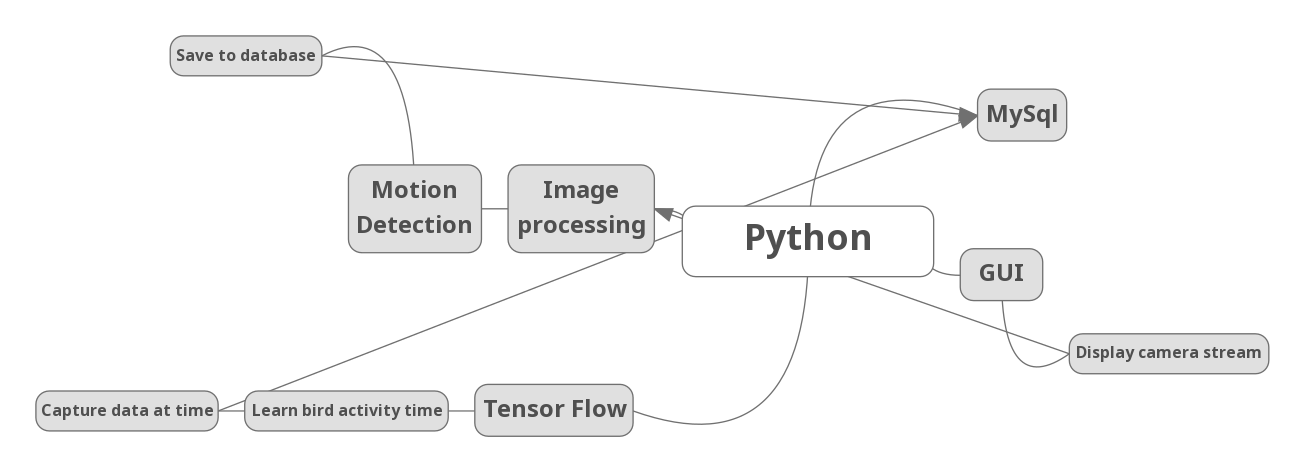
\includegraphics[scale=0.3]{img/mindMap.png}
       \caption{Research Mind Map}
       \label{fig:my_label}
       \end{figure}
 \subsection{Python}
 I began my software research with the programming language I would be basing the program on. I began by watching the 'Python for Beginners' course~\cite{pythonForBegin} in my free time, building my grasp on the language before moving to more complex portions.  Once I believed I had gained an adequate grasp of the language I investigated how to get camera input which lead me to find OpenCV~\cite{openCV}, while researching OpenCV I learned that it was included in a large collection of useful libraries called Anaconda~\cite{anacondaLibs}. I installed Anaconda as a convenience, believing it would be easier to install them as a package, rather than each extra library I would need one by one. I also came to learn that python is one of the slower languages, which surprised me due to it's popularity.  
  \begin{figure}[!htbp] 
      \centering
     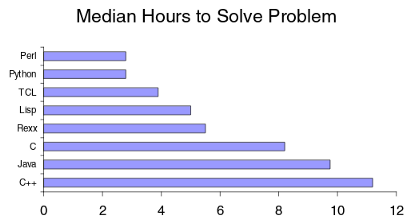
\includegraphics{img/pythonSlow.png}
      \caption{Chart displaying programming language speeds}
      \label{fig:my_label}
  \end{figure}    

I planned to use a Graphic User Interface (GUI) to control and display the program, because it is also something I have little experience in. This lead me to find tkinter, which is Pythons standard GUI developing method~\cite{tkinter}. I learned to create basic windows and how to style them. This feature was later discarded, in favour Flask.
 \subsection{OpenCV}
 I tried to learn OpenCV by searching the documentation for functionality I thought would be relevant to the project, however this proved to be inefficient as I found them somewhat difficult to understand without a proper explanation. As a  result I turned to youtube for a brief explanation, however I found an extremely helpful and extensive video course on OpenCV ~\cite{openCVCourse}, I also discovered and article on color manipulation and drawing on images which later made it easier to implement the motion detection~\cite{openCVArticle}. While researching OpenCV I learned of Imutils, an anaconda library which contains some convenient functions, making some OpenCV tasks less complicated~\cite{imutils}.
 \subsection{Motion Detection}
 Once I had learned how to capture the camera stream in Python I moved onto motion detection. I decided to learn the basics of how motion detection worked, since I my knowledge in the field was negligible. I learned that Computer Vision motion detection, the type I would be implementing. Revolves around the program getting a frame, storing it and then comparing any changes in pixels with the next frame(s)~\cite{howMotion}. Upon reading this I implemented a simple algorithm that:
 \begin{itemize}
 \item Read in an initial frame.
 \item Stored that frame.
 \item Read the next frame(s).
 \item Directly compare the two frames.
 \item Returned the last frame if movement was detected.
 \end{itemize}
 This algorithm was both disappointing and exciting, on one hand I had a motion detector that returned an image if a single pixel changed, on the other hand I had a motion detector, albeit a barely functioning one. To fix this I investigated how to remove the background and desensitize the comparison. That lead me to find out about OpenCV's built in background detector, \verb|cv2.BackgroundSubtractorMOG2~\cite{backgroundSubtract}|. I was amazed at how well it worked. I was also amazed at how much processing power it consumed. On the single camera I seen my CPU (Central Processing Unit) usage climb by 40 percent. I knew this couldn't be usable on the Raspberry Pi's weaker processor, especially when I had to incorporate more than one camera. However the openCV image detailing background subtraction made things easier to understand.
 \begin{figure}[!htbp] 
      \centering
     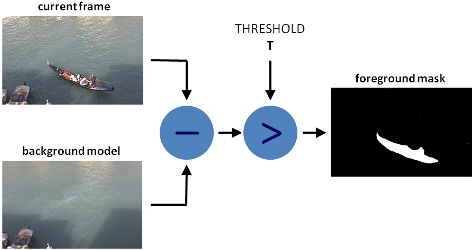
\includegraphics[scale=0.6]{img/backgroundSub.png}
      \caption{Background subtraction explained}
      \label{fig:my_label}
  \end{figure}    
\\ From what I understood of this, the first frame read in would be the background frame and the next frame read would then be subtracted from the background frame. What was left after the subtract would then be made into the foreground mask if a certain number or 'threshold' of pixels were changed. I then tried out some rough code:
 \begin{itemize}
 \item Read in an initial frame.
 \item Stored that frame.
 \item Read the next frame(s).
 \item Directly compare the two frames.
 \item Add the difference to a mask frame 
 \item compare next frame to the mask frame
 \item Returned the last frame if movement was detected.
 \end{itemize}
 This code worked better but it wasn't what I needed, it picked up too much noise from the camera, which it interpreted as movement. To fix this I looked up ways to remove camera noise. While browsing the OpenCV docs for a solution, I found the \verb|'cv2.GaussianBlur'| function, Gaussian blur is a soft blur so I hypothesized that it would fix the noise issue. After some trial and error I found it was best to create a blurred frame and use that, rather than blur the mask. While testing the blur, I noticed that when the colours of fans on my computer changed, it would also trigger the motion detection, to fix this I created a grey scale frame using \verb|cv2.cvtColor().| The motion detection was now working rather well. However I noticed that if something came into frame of the camera, that wasn't there when it was initialed, that it would constantly detect motion. To remedy this I implement a simple loop that sets the background frame every second, with this my motion detection was now finished.    Code Snippet:\begin{verbatim}
        if currentTime > self.lastMovementTime + timedelta(seconds=1):  
            	self.initialFrame = grayFrame 
            	self.lastMovementTime = datetime.now() 
            	self.movementDetected = True 
 \end{verbatim}
 
\section{TensorFlow}
TensorFlow is a Python library developed by google, which provides and open source AI framework. I was introduced to TensorFlow by Dr. Ian Mcloughlin's module Emerging Technologies, this module gave me a good basis for the Keras neural network. I researched and considered adding a neural network to track the times of day when motion is detected~\cite{kerasTrain}. I shelved this idea as I felt it would push the scope of the project too far, instead focusing on refining the at the time, primitive motion detection.

\section{Remote Connection}
Late into the development cycle I realised that it would be best to be able to access the program externally, due to their remote locations. It would optimal to sporadically check the program, to ensure the cameras had not been damaged or moved. To do this I initially considered leaving the program as is and to a run SSH (Secure Shell) to control the Pi. However after using Flask in the Emerging Technologies module I decided it could be worth while implementing a web server, so that the user access the program from anywhere, not just a computer (Example: Their phone).

\section{Flask}
After briefly exploring the Flask web framework in the Emerging Technologies module, I decided to succinctly read through the documentation for any functionality I deemed necessary~\cite{flask}. While researching Flask I found out about Django, another Python web development framework however after some further research I decided that I would stick with Flask as it is more lightweight~\cite{flaskVDjango} and resource management was big concern for this project. Once certain I found two extensive Flask video courses, which helped my understanding greatly~\cite{flaskCourse}~\cite{flaskCourse2}. I noticed in the Flask Docs there was an included authentication library that simplifies authentication. The BasicAuth library and it's function, can require specified views to require authentication to access, by adding the line
\verb|"@basic_auth.required"| after the app route, you can also force the entire application / site to require authentication by using the command \verb|"app.config['BASIC_AUTH_FORCE'] = True"|
\section{MySql}
 I researched MySql integration with Flask and found  \verb|"Flask-MySQL"| and \verb|"SQLAlchemy"|, upon further research  \verb|"SQLAlchemy"| seemed to be the best supported option of the two, though they both added SQL database functionality. However due to previous projects using database management systems, I felt competent in these areas and did not feel the need to add them. I wished to store the files directly to the device so that they could easily be retrieved by the user, should they wish to copy from the directory to another etc. This turned out to be easier than expected. In context of the program saving follows the following format: \verb|"cv.SaveImage(directory+filename, image)"| and retrieving the file in the program follows: \verb|os.read(directory to file)"|
\chapter{Methodology}
During the development the development of this project I adopted the Agile development methodology, as well as Function driven development. I used these methods to organize sprints for myself, in which I developed a certain function.
\section{What is Agile Development}
The Agile development methodology is an iterative approach to development, instead of developing the product in a linear 'Big Bang' approach. Agile development incorporates customer collaboration, teamwork and the ability to adapt and overcome issues. Agile development promotes sustainable development~\cite{agileManifest}
 \begin{figure}[!htbp] 
     \centering
     
\includegraphics[scale=0.5]{img/agile.jpg}
     \caption{Agile Development diagram}
     \label{fig:my_label}
 \end{figure} 
\section{Why I chose Agile}
I chose agile development as it allowed me to research and develop code in relays. I could research for some days and then develop for the next amount of days, allowing me to develop features as I see fit, being able to take time to research some of the more onerous tasks, while developing another task. I found it to a great change over my usual Linear design method, I no longer had to research, develop and test one task at a time. I could partially develop, stop and revisit as I seen fit.
\section{What is Function Driven Development}
Function Driven Development is an agile development method, it centers around prioritising development on features. The team / developer develops an overall model for the project then build a features list. They then develop feature by feature.
\section{Why I chose Function Driven Development}
I chose Function Driven Development primarily as I wanted to experiment with a different development approach, generally I utilize Test-Drive Development, where I do not move on to the next feature until the current feature works flawlessly with the previous implemented features. For this project I chose to develop the features separately.
\begin{itemize}
    \item Develop Camera Capture
    \item Develop Motion Detection
    \item Develop Image capture on Motion Detection
    \item Develop Provisional GUI
    \item Develop Flask Application
\end{itemize}
\section{Version Control}
I did not implement an external version control such as Github for this project. As I was developing I would develop the function on my desktop and once it was completed I would deployed it to the Raspberry Pi for performance testing. If it passed the performance test then it would remain on the Pi, while I iterated on the copy on my desktop. I did not feel Git was necessary as I developed a function fully almost every sprint. These functions were not packaged together to form the complete application until the end of the development cycle.
\section{Time Management}
\subsection{Workload}
I feel I managed my workload for the first semester quite well, I dedicated every project a time-slot for the week and stuck to it quite well. My workload for this project was one to two hours research on Mondays and two Hours development on Tuesdays. I stuck to this weekly until the very end of the semester where it was forced to a bi-weekly to accommodate other deadlines. My time management for the second semester however was lackluster. Due to health issues at the start of the year I did not stick to my initial plan and generated a backlog that I carried for a large portion of the semester. The backlog and scope creep of other projects ended up resulting in a few coding sprints where I would focus on just one project rather than spreading it equally.

\chapter{Technology Review}
In this chapter I will review the technologies used in this project, breaking them down and discussing in detail how they are used and why I chose them.
\section{Languages}
\subsection{Python}
Python is a high level, interpreted programming language, that aims to cut time spent figuring out things such variables and objects, so that you can focus on developing your program. The fact that python is an interpreted makes it rather forgiving, automatically raising exceptions and the like. Python also does not require a compiler, instead it can be run straight from the command line. Python has a massive pool of readily available libraries that add many niche and quality of life functions. Python however suffers from slow speed as it is interpreted instead of compiled. I chose Python for this application because of it's extensive libraries, great support for Linux based operating systems and my own personal curiosity about the language as my experience before this project was minuscule.~\cite{python}
\begin{figure}[!htbp] 
    \centering
    
\includegraphics[scale = 0.1]{img/python.png}
    \caption{An example of python code}
    \label{fig:my_label}
\end{figure}

\subsection{HTML}
HyperText Markup Language or HTML is the standard markup language for creating Web sites. It is the structure of the web page. HTML consists of numerous elements and tags, all of which describe to the browser how it should display the site correctly. HTML is a versatile, consistent language that is at the core of almost every web application. For this reason HTML was necessary to display my web app~\cite{html}

\subsection{JavaScript}
JavaScript is a scripting language that allows you to dynamically update content and input data, along with a whole slew of other functions within HTML. 
JavaScript is closely tied to both HTML and CSS. Java script was used for this project to assist with flask and HTML core functionality.
\begin{figure}[!htbp] 
    \centering
    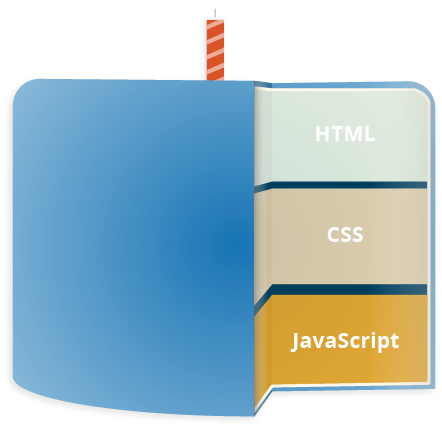
\includegraphics[scale = 0.35]{img/cake.png}
    \caption{The HTML, JavaScript, CSS Stack.}
    \label{fig:my_label}
\end{figure}

\subsection{Cascading Style Sheets (Css)}
Cascading Style Sheets or CSS is a language that allows the user to completely change the looks of their web page. Css is used to design HTML to look a certain way. I had to include css to make the web application aesthetically pleasing. 
\begin{figure}[!htbp] 
    \centering
    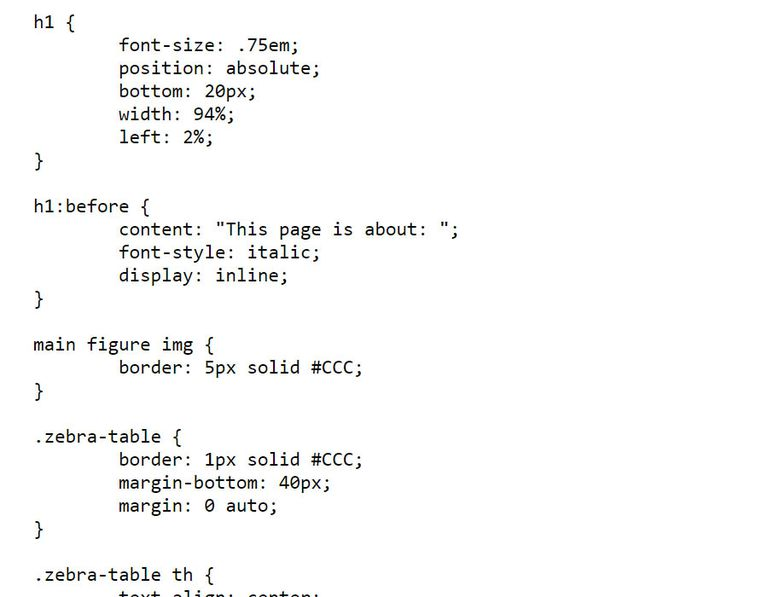
\includegraphics[scale = 0.7]{img/css.jpg}
    \caption{css Source code example.}
    \label{fig:my_label}
\end{figure}

\section{Libraries}
\subsection{OpenCV}
OpenCV is an open source library dedicate to image processing and computer vision. OpenCV is short for Open Source Vision Library. Since motion detection is a product of computer vision and openCV is available for Python it made sense to utilize it. Many functions of the project relied upon the openCV library. Example: Getting the camera input. OpenCV is not without it's faults however, as the BackgroundSubtract function is not well optimised, consuming huge ammounts of CPU resources, too much for the Raspberry Pi to handle, thus making it unusable. ~\cite{openCVAbout}
\begin{figure}[!htbp] 
    \centering
    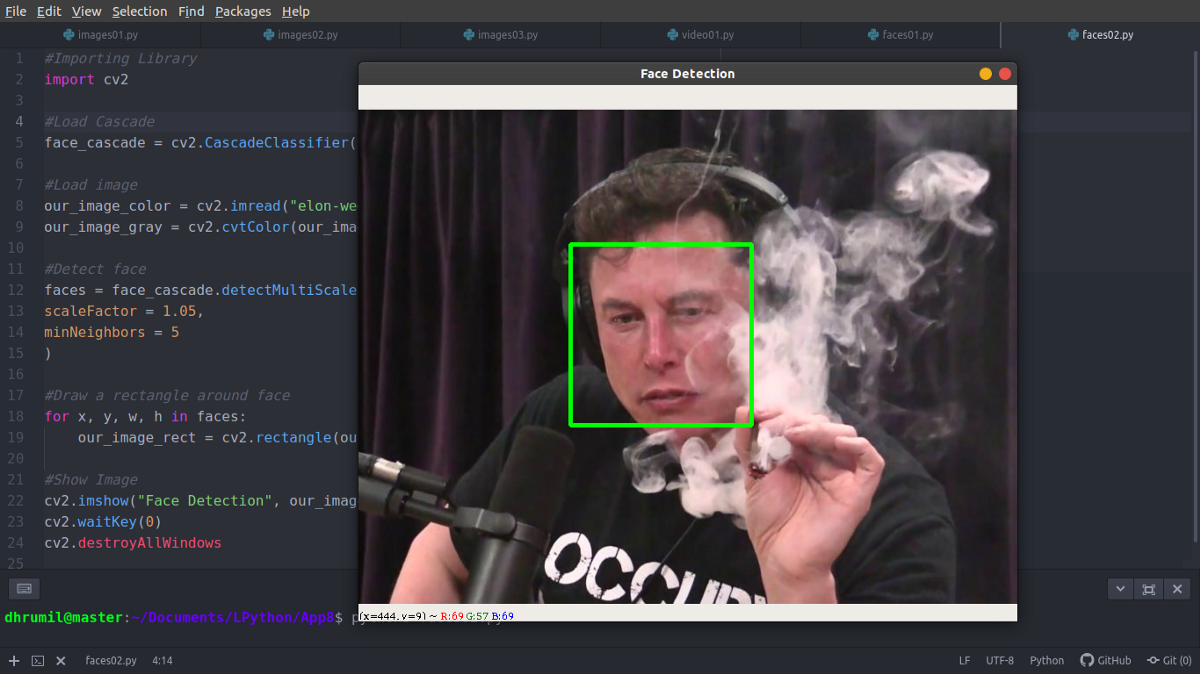
\includegraphics[scale = 0.35]{img/openCV.png}
    \caption{An example of openCV python code and at work}
    \label{fig:my_label}
\end{figure}
\subsection{NumPy}
Numpy is a highly optimised, powerful scientific computing library for Python. I used NumPy in this project for it's array handling capabilites as well as it's transform functions.~\cite{numpy}

\section{Framework}
\subsection{Flask}
\begin{figure}[!htbp] 
    \centering
    
\includegraphics[scale = 0.35]{img/flaskLogo.png}
    \caption{Flask logo}
    \label{fig:my_label}
\end{figure}
Flask is a lightweight web framework platform written in Python. It is lightweight, classified as 'microframework' as it does not require any particular libraries. Flask was essential for me as it is less resource intensive and easier to learnt than Django. I based the entire application around Flask. Flask has a built in web development server, however it is recommended to deploy to a dedicated server. For this application I chose Gevent.~\cite{flaskDeploy}
\chapter{System Design}
\section{Intro}
In this chapter I shall discuss the initial system design, final system design and project architecture 
\section{Initial Design}
 \begin{figure}[!htbp] 
     \centering
     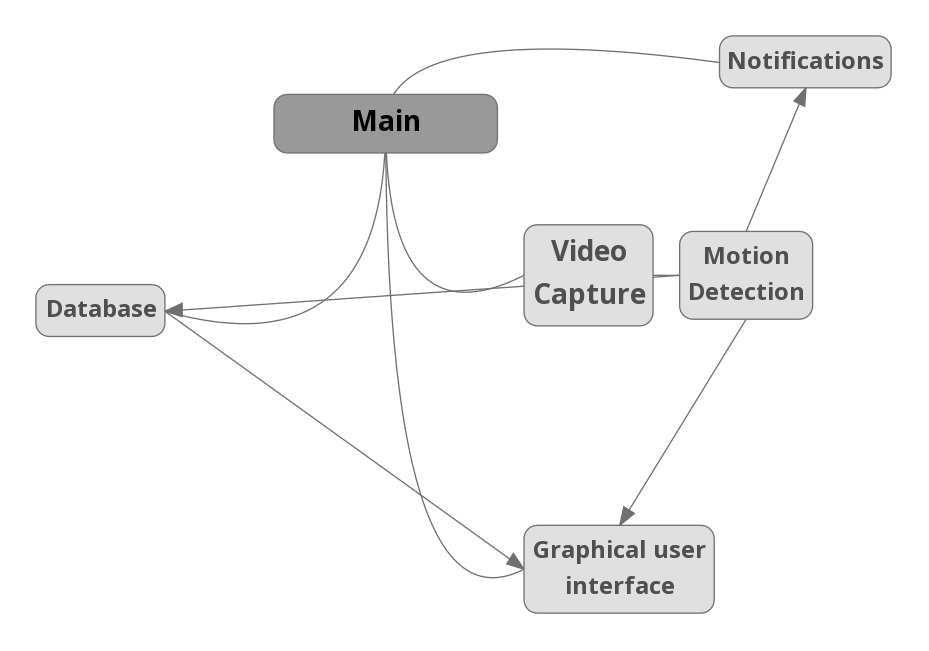
\includegraphics[scale=0.4]{img/initialDesign.png}
     \caption{Initial System design}
     \label{fig:my_label}
\end{figure}
Initially I designed the program to be executed locally and to run until user termination, detecting motion, storing the frame of motion. However I wasn't satisfied with the program simply saving the data, I wanted to be able to see and interact with it. I created a mock up graphical user interface after I had finished the core functions. Motion detection, saving images etc.
     \begin{figure}[!htbp] 
         \centering
         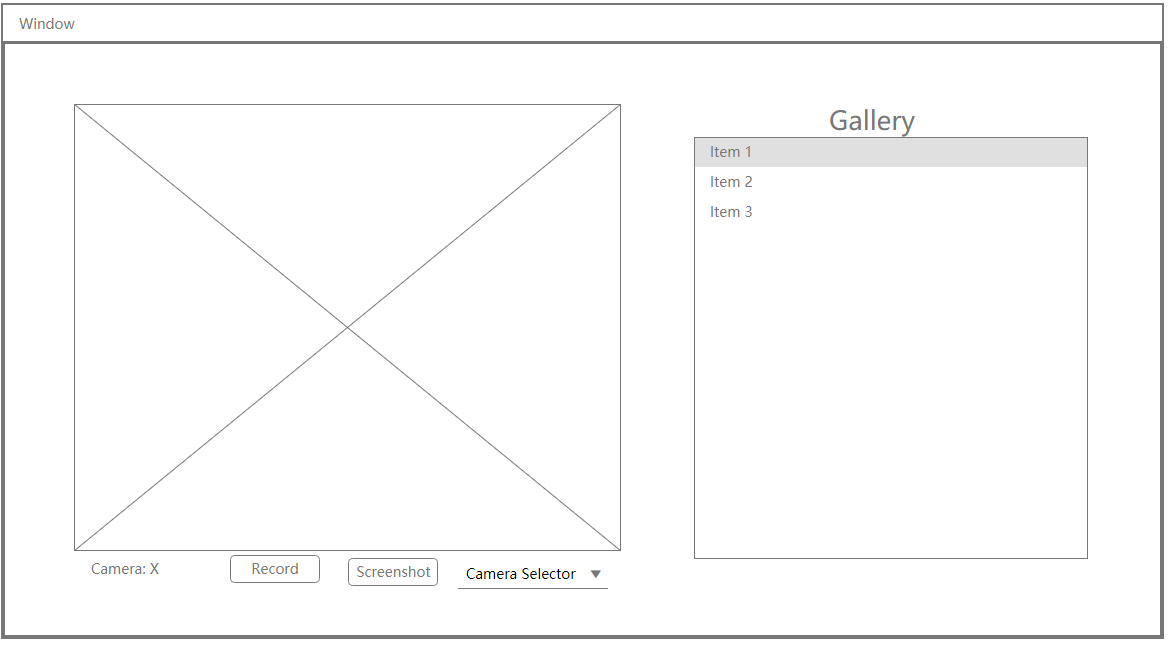
\includegraphics[scale=0.5]{img/InitialUI.PNG}
         \caption{Initial User-Interface mockup}
         \label{fig:my_label}
     \end{figure}    
    \subsection{Initial Architecture}
    The initial project project was designed to be executed from a main.py file. Which would instantiate X number of cameras. When movement was detected it called the send email function, passing the frame captured at that moment. Files were passed to an SQL database and stored as blob files.\\
    There was no GUI, the program would run. Display the camera stream in a frame while running.
    Once I began to design the GUI I made the choice to convert to a Flask app and remove the need for SSH
    \section {Final Design}
    \begin{figure}[!htbp] 
        \centering
        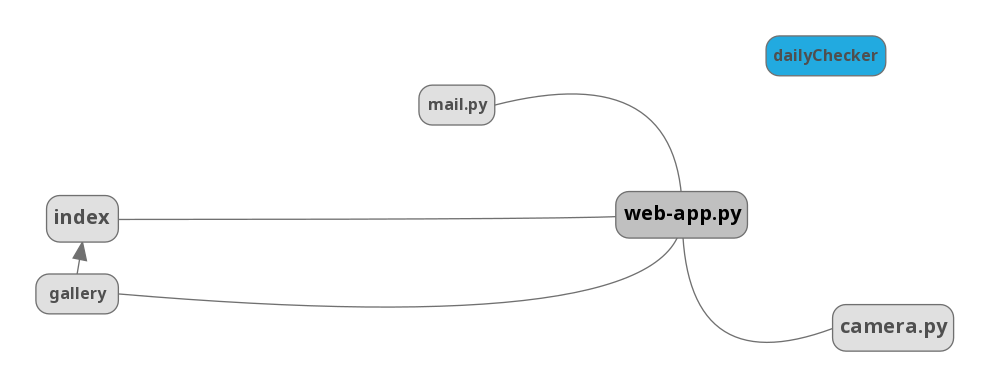
\includegraphics[scale=0.4]{img/currentDesign.png}
        \caption{Current Design}
        \label{fig:my_label}
    \end{figure}    
    \subsection{Final Architecture}
    The final design architecture remains similar to the first albeit with a few meaningful changes.
    The final architecture still runs from the main: web-app.py. This instantiates two of the camera class. It runs on 0.0.0.0:5000 to allow for external access, on a gevent WSGI server. web-app.py has 4 routes. 
    \begin{itemize}
        \item \verb|('/')'|: Returns the index/stream page, this page displays the live streams of both cameras.
         \item  \verb|('/gallery')'|: Returns the gallery page, which displays all the images currently save in the "static/gallery" directory.
         \item \verb|('video_stream')'|: Returns the live video stream of the first camera. This is used to route the stream to the index.
          \item \verb|('video_stream2')'|: Returns the live video stream of the second camera. This is used to route the stream to the index
    \end{itemize}
   The web-app.py calls the mail.py and passes it an image. The email script takes this image and uses smtplib which creates an SMTP connection and sends the email to the user defined email address.\\SMTP stands for Simple Mail Transfer Protocol, used to send emails\cite{SMTP}\\An example of the script run without passing an image:   
   \begin{figure}[!htbp] 
       \centering
       
\includegraphics[scale=1]{img/ssEmail.PNG}
       \caption{Screenshot of the default email script result}
       \label{fig:my_label}
   \end{figure}    
  
   The unimplemented dailyChecker uses geopy.geocoders to receive the geocode on the location defined in the program, in this case Galway. It passes this geocode to the sunrise api. This api takes the geocode and calculates the sunrise and sunset for that day at that location. However the format it returns is not compatable to be compared. This was going to be used to compare against current datetime and if the two matched, then take a screenshot from both cameras. \\ A screenshot of the code running in command line: 
   \begin{figure}[!htbp] 
       \centering
      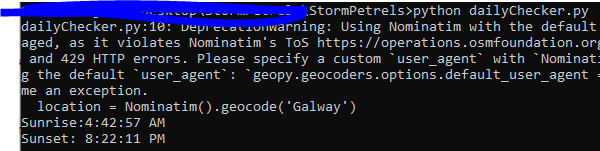
\includegraphics[scale=1]{img/ssDailychecker.PNG}
       \caption{Screenshot of the daily checker script working}
       \label{fig:my_label}
   \end{figure}    
  
    The camera.py contains the vast majority of the programs functionality and logic. \\The class must be initialised, in this case through the web-app.py. Once initialised the camera will run the get movement function. While this function is running the camera constantly reads in frames. The most recent frame is converted to grayscale and blurred to reduce image noise. If there is no initial frame then, it is set to the gray frame. This is to get our background. Then the initial frame and gray frame are compared and output to a deltaFrame which is then thresholded, which means if a pixel in the particular image is greater than a certain value then it is converted to flat white, if it's below it is returned flat black.\cite{openCVThresh}. The image is then dilated which fills in the holes/gaps of the threshold. \\ Then using cv2's findContour function the program adds all contours to an array. Then it reads the contours fro the array and draws the rectangle over the area where the contour is greater than 1000 \\ That is the basic algorithm for motion detection. \\ If there is motion detected then the program saves the copy of the frame that hasn't been modified to a jpg file and starts a countdown. The program cannot take another picture from the camera instance until the timer has finished, this prevents endless streams of motion detection being output.\\ If motion is detected and the camera is not currently saving a video, then a 10 second video after the motion is detected should be saved.
      \\\\I removed the SQL database as I felt it was not needed, I thought it was more user friendly to store the images in the static/gallery directory. 
     \begin{figure}[!htbp] 
         \centering
         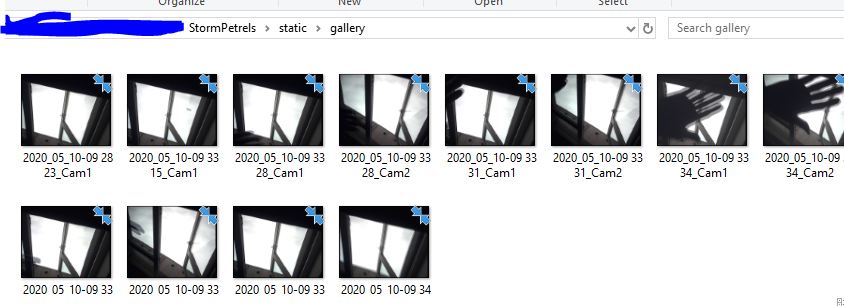
\includegraphics[scale=1]{img/gallery.PNG}
         \caption{Screenshot of the Gallery directory}
         \label{fig:my_label}
     \end{figure}   
\subsection{Application Design}
    \begin{figure}[!htbp] 
            \centering
             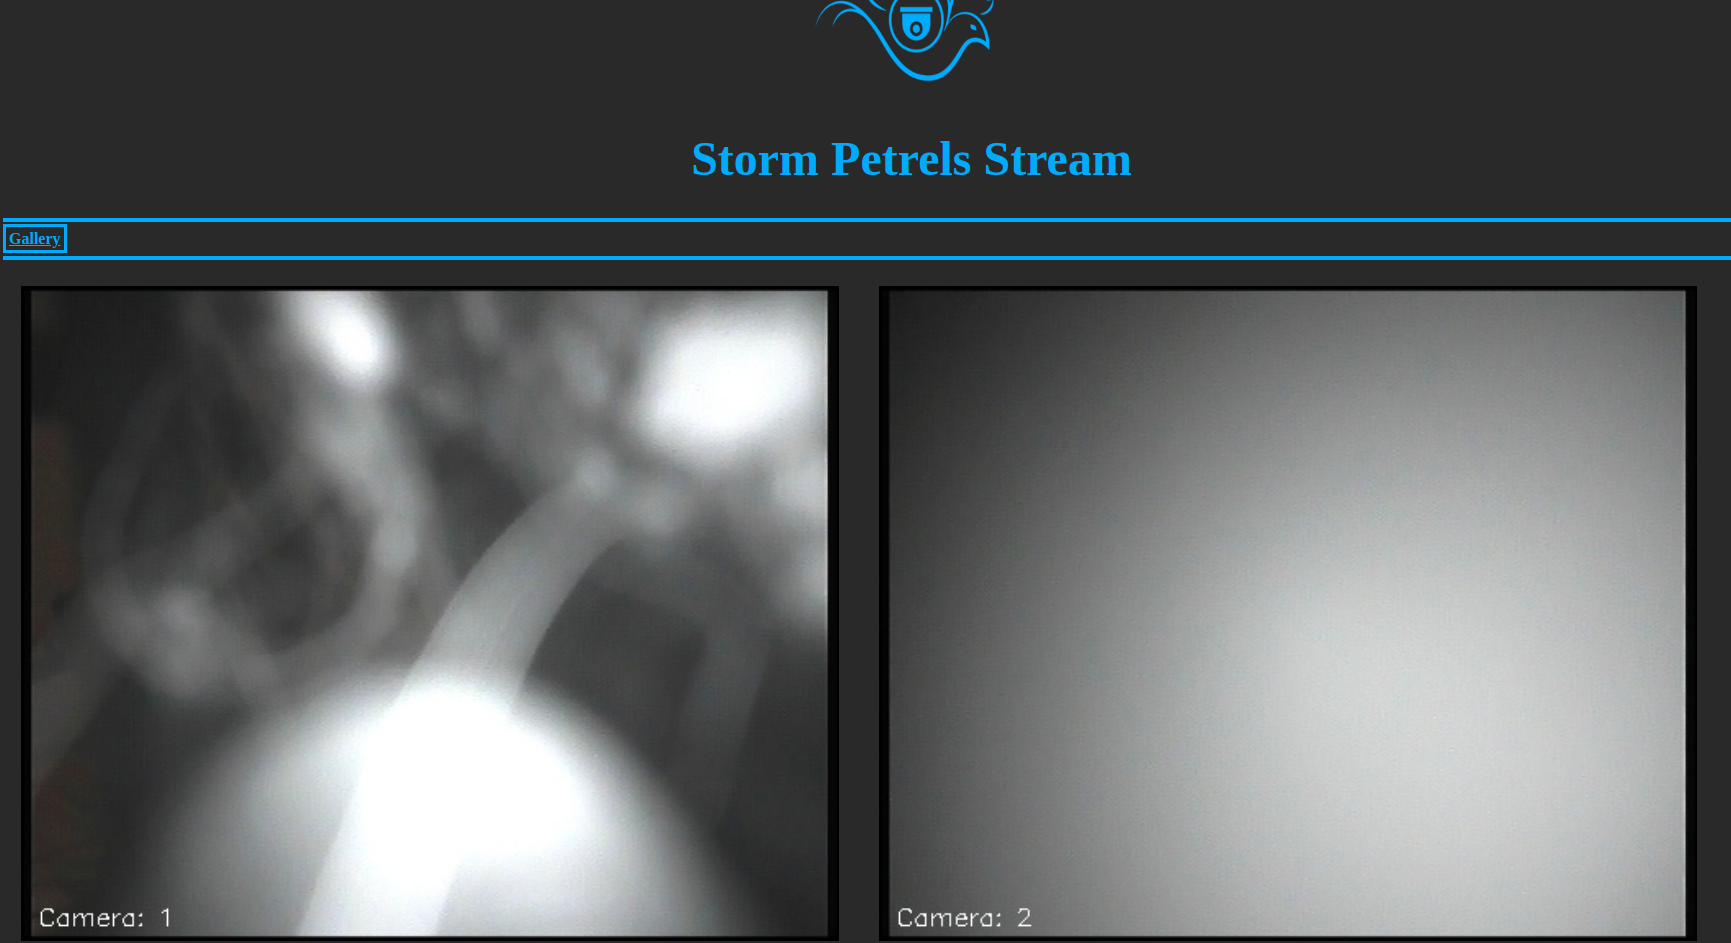
\includegraphics[scale=0.25]{img/ssStream.png}
            \caption{Screenshot of the Index page}
            \label{fig:my_label}
        \end{figure}    
    \begin{figure}[!htbp] 
                \centering
                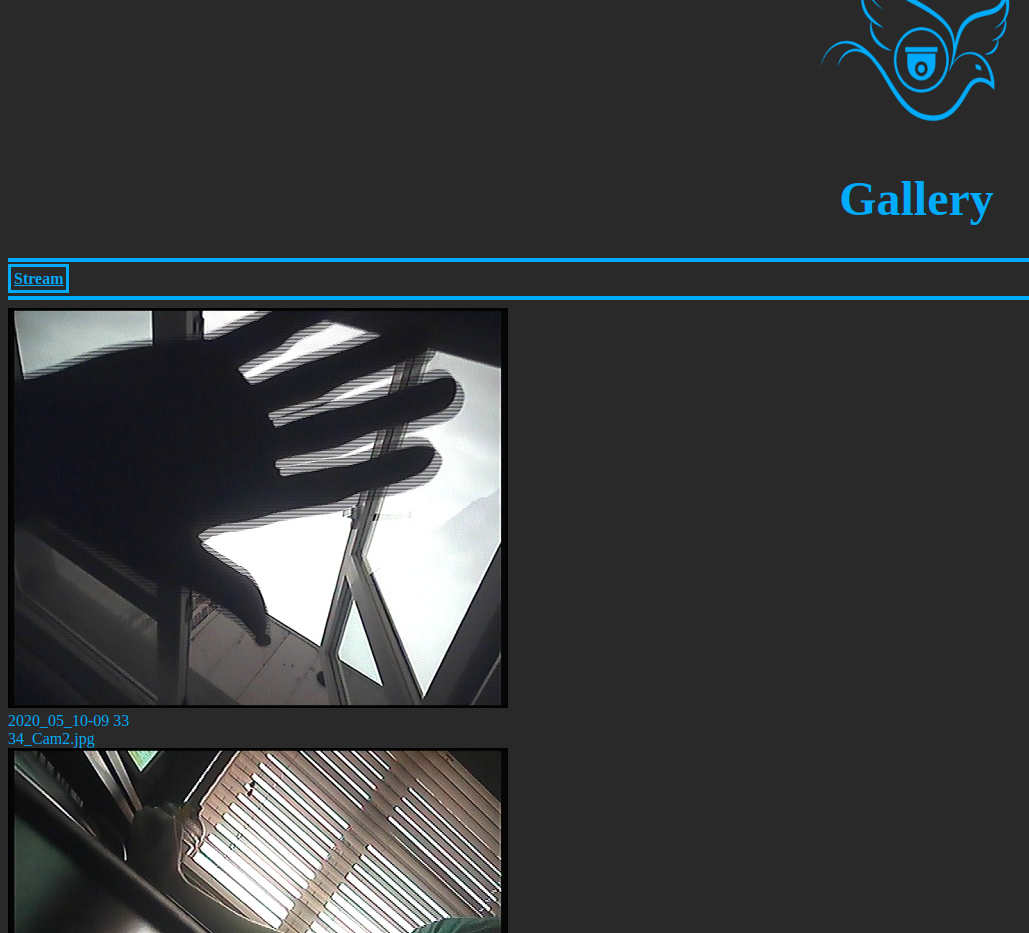
\includegraphics[scale=0.4]{img/ssGallery.png}
                \caption{Screenshot of the Gallery page}
                \label{fig:my_label}
            \end{figure}  
\chapter{System Evaluation}
After porting my program to Flask I have tested the application extensively and can conclude that I am not satisfied with how robust it is. However I am happy with it core functions.
\section{Known issues}
\begin{itemize}
\item Camera's will not restart if signal is dropped. If the camera feed is lost from the data or power cable and then comes back it is fine, however if the capture card encounters and issue, the stream will end. This does not crash the program it simply stops the stream for the camera in question. I have been unable to implement a method to restart said camera. Pseudo code tested: "if camera(X) == null, wait 5 seconds, re-intialize camera(x)".
\item Camera cannot save to video file, cv VideoWriter instantiates fine, but after the loop time to write video, it returns an invalid .avi file. Consulted stack overflow, matched the frame sizes and other possible fixes ,suspected codec error, possible write permissions issue. error\cite{stackOverflow}\cite{stackOverflow2}.
\item If deployed to the Gevent server, app will function fine but can randomly become stuck on the index / stream page, unable to navigate or load the gallery page. Issue not present on the flask development server. Suspected threading issue.
\end{itemize}

\section{Efficiency}
I am pleased with the projects efficiency, while processing the images in real time, the task consumes less than \verb|20% cpu usage| on my aging processor. It does push the Raspberry Pi a lot harder, however there is no frame rate drop or any other performance issues. \\ The file size of saved images is quite low too, averaging around 44KBs per image. This is great for storage, as the program could be run for weeks on end without fearing that it would fill up the 64Gb SD card inside of the Raspberry Pi. \\ The only efficiency area I am not pleased with is the network bandwidth. When running locally, the program is fine, however I tested the external connect ability of the app, by forwarding the necessary ports on my router and logging into the application from outside my network, using my phone. Upon doing this I seen in my computer's resource manager that my network activity spiked from mere Kbp/s to a constant average of 3.6Mbp/s. This is not good as if the app is to be deployed remotely using a 4G dongle, then a data rate similar to that would burn through any Data plan / 'Fair Usage Policy'.

\section {Ease of Use}
This application is easy to setup and use. The readme is sufficient, the requirements.txt contains all necessary requirements, the easy way to install them is included in the readme : 'pip install -r requirements.txt'. Once the application is running all the user has to do is visit the index and check if the camera's are working, the program will run and collect data by itself. \\ The code is sufficiently commented, so that if the user must change any variable, they will have a clear idea which to change

\chapter{Conclusion}
This conclusion will briefly recap and review the project. I will compare the delivered project to the brief, my goals for the project, break down possible short comings, outline possible refinements, what I would do differently and give my personal reflection on the project.
\section{Objective of the project}
The brief requested a system that can be remotely deployed to remote locations to capture still images of birds by motion sensing and programmable intervals. The project delivered an application that can be remotely accessed, records still images based on motion detection. I took some liberty with the programmable intervals, I believed that the sun rise and sun set timing retrieved from the API would suffice, as they are times of high activity in birds. However adding a programmable timer would be relatively simple to implement with some ['GET','POST'] request methods on the index.
\section{My goals for the project}
My goals for the project were as follows:
\begin{itemize}
    \item Deliver a program based on the brief.
    \item Expand my Python knowledge.
    \item Learn more about Flask.
    \item Learn about web servers.
    \item Get more experience in Graphical User Interfaces.
    \item Learn how to program motion detection.
    \item Improve my time management skills.
\end{itemize}
I have met most of my goals for this project. I delivered a program matching the brief, however I would like it to be more robust before actual deployment. \\ I met my learning goals. My time management improvement was successful for the first semester, however I let it slip in the second semester.
\section{Shortcomings}
The following are all the shortcoming in regards to the project in my opionion:
\begin{itemize}
    \item No video recording.
    \item Sun time API didn't work.
    \item Email implementation does not work properly in current state.
    \item Network bandwidth is too high.
    \item Camera needs to be able to be restarted if feed is lost. However I believe this issue is based on the capture card
\end{itemize}
\section{Possible improvements}
\begin{itemize}
    \item Enable the video recording.
    \item Manually screen shot and record video from the stream page.
    \item SSH implementation on the server.
    \item Fix network bandwidth.
    \item Possibly add button to restart or instantiate new cameras.
    \item Delete items from gallery page.
\end{itemize}
\section{What would I change}
The self hosting server was influenced by the low cost element of the brief. If budget was to allow it, I would have created a server client that is hosted in the cloud, that reads streams from the client program, which is deployed on the Raspberry Pi. The server side application would read in the streams and do the computations, as well as storing the files. This could be achieved using Flask and sockets.
\begin{itemize}
\item Briefly summarise your context and ob-jectives (a few lines).
\item Highlight your findings from the evalua-tion section / chapter and any opportuni-ties identified.
\end{itemize}
\section {Reflection}
I found this project to be both interesting and challenging simultaneously, the motion detection and other such CV2 commands were fun to test out and try to implement. I have definitely expanded my knowledge on Python and it's many libraries, and while it has it's uses I have come to the conclusion that it is not as enjoyable to work with when compared to other coding languages such as Java or \verb|C#|. The  no variable names and indentation takes a lot of getting used to. I am mostly happy with the project I have delivered. I feel I have made a good foundation, save for the few notable shortcomings. I am personally disappointed with my own time management skills and will continue to work on them. \\
To close, this project was a definite challenge but a worthwile one that I am happy I have completed. 

\chapter{Appendices}
\href{https://github.com/Jakecw97/FinalYearProject}{GitHub: https://github.com/Jakecw97/FinalYearProject}\\
\href{https://youtu.be/L1AUL8wypps}{Screencast: https://youtu.be/L1AUL8wypps}
  \bibliographystyle{ieeetr}
  \bibliography{bibliography}
\end{document}
